\section{Part~VI: Conservation Law Audit}\label{sec:part6}

Pointwise relative $\Ltwo$ error is overwhelmingly the dominant performance metric in the physics-informed neural network literature. While mathematically convenient for establishing basic convergence, this scalar metric fundamentally fails to capture the underlying physics. Physically meaningful solutions must not only approximate the correct scalar field pointwise but also strictly satisfy the global macroscopic conservation laws dictated by the PDE. In this section, we rigorously audit four distinct physical invariants across six unique training configurations—spanning from optimal success to various isolated failure regimes—to determine if structural failure manifests uniquely in conservative metrics, and whether these metrics expose hidden flaws in seemingly successful models.

\subsection{Invariant Definitions}\label{sec:exp24}\label{sec:exp26}

To quantitatively assess physical fidelity, we evaluate four primary global integral invariants, denoted as $C_1$, $C_2$, $C_3$, and $C_4$. The $C_1$ metric directly measures the global mass conservation violation, representing the deviation of the spatial integral from the prescribed initial mass over time. $C_2$ measures momentum and energy conservation violations, tracking the $\Ltwo$-norm temporal drift of the system against theoretical bounds. Furthermore, we include \textbf{C3 (Entropy Proxy):} A strictly convex entropy functional utilized to measure non-physical dispersion and artificial shock formation, defined analytically as $C_3(t) = \int_{\Omega} u^2 \log(|u| + \epsilon) \,dx$, where $\epsilon = 1 \times 10^{-8}$ is applied to avoid the singularity at $u=0$. We also evaluate $C_4$, which enforces the strict mean boundary flux imbalance. A structurally sound PINN architecture should theoretically drive all these continuous integral violations exactly to zero as the localized PDE residual is continuously minimized. Failure to do so indicates that the network is memorizing localized patterns rather than learning the generalized physical operator.

\subsection{Audit Results}\label{sec:exp26_results}

This section synthesizes findings from two distinct but related experiments: Experiment~26, which performs the comprehensive conservation law audit across all six failure modes, and Experiment~24, which specifically isolates the phenomenon of silent conservation leakage in seemingly successful models. The results of the broader invariant audit (Experiment~26) across the isolated failure modes are summarized below. (Note: FM4 is drawn from a low-stiffness Burgers configuration, $\nu=0.1$, to serve as an initialization-sensitive outlier.)

\begin{table*}[htpb]
    \centering
    \caption{Global conservation law violations across six identified training regimes.}
    \label{tab:exp26_conservation}
    \begin{tabular}{@{}llrrrr@{}}
        \toprule
        FM & Description & $\Ltwo$ Error & $C_1$ Violation & $C_2$ Violation & Mean $C_4$ Flux \\
        \midrule
        FM1 & Spectral Bias & $0.938$ & $103.46$ & $0.980$ & $0.263$ \\
        FM2 & Success Control & $0.025$ & $33.48$\textsuperscript{a} & $0.005$ & $1.367$ \\
        FM3 & Gradient Pathology & $0.888$ & $27.24$ & $0.999$ & $0.226$ \\
        FM4 & Initialization-Sensitive Outlier ($\nu=0.1$, Burgers)\textsuperscript{b} & $0.215$ & $47.63$ & $0.903$ & $0.001$ \\
        FM5 & Collocation Starvation & $0.660$ & $7.75$ & $0.996$ & $0.522$ \\
        FM6 & OptimStagnation & $0.930$ & $689.67$\textsuperscript{c} & $0.981$ & $0.240$ \\
        \bottomrule
    \end{tabular}
    \begin{flushleft}
    \textsuperscript{a}FM2 (Success Control): the $C_1$ mass violation of $33.48$ reflects antisymmetry drift in the periodic advection solution rather than a physically meaningful mass error; see Section~8.2 for discussion.\\
    \textsuperscript{b}FM4 exhibits an unexpected $\Ltwo \approx 0.215$ despite the low-stiffness configuration ($\nu=0.1$). This anomalous result is classified as an initialization-sensitive outlier and is retained for completeness; conservation violation metrics reflect this partial failure state and should be interpreted accordingly.\\
    \textsuperscript{c}The $C_1$ mass violation for FM6 ($\approx 689.67$) is anomalously large relative to the other failure modes. At $\Ltwo \approx 0.930$, the shallow network predicts a near-constant non-zero function due to capacity limitations, rather than the zero function; the mass integral of this constant over the domain produces a large absolute $C_1$ deviation. This is an artifact of the near-constant non-zero prediction mode rather than a physically meaningful mass conservation violation.\\
    The invariants are evaluated precisely at the boundary endpoints or integrated over the continuous spatial domain. To verify that the reported integral violations are genuine network pathologies rather than quadrature artifacts, we conducted a spatial grid convergence study. The continuous integrals $C_1$ and $C_2$ were evaluated using the composite trapezoidal rule on a highly resolved uniform spatial grid of $N_x = 512$ points. Systematically doubling the resolution to $N_x = 1024$ and $N_x = 2048$ yielded identical violation measurements up to the fifth decimal place, confirming that the numerical integration error is strictly negligible relative to the severe $\mathcal{O}(10^{-1})$ conservation failures generated by the PINN approximations themselves. All reported violations are absolute errors normalized against the exact or initial-condition reference states.
    \end{flushleft}
\end{table*}

Experiment~24 (Silent Conservation Leakage) provided the initial evidence for this decoupling. Comparing the baseline Spectral Bias model (FM1) against the highly optimized Success Control (FM2) reveals critical, counter-intuitive insights into neural network behavior. While the successful model (FM2) effectively drives the $C_2$ momentum violation to a near-zero magnitude ($0.005$) compared to the severe violation present in FM1 ($0.980$), FM2 exhibits an unexpectedly large $C_1$ mass violation of $33.48$. For periodic advection, the exact analytical solution integrates identically to zero across the spatial domain; deviations in $C_1$ reflect the PINN's explicit failure to maintain this antisymmetry, which is a separate pathology from $\Ltwo$ accuracy entirely. The network manages to achieve extremely high pointwise precision while simultaneously drifting significantly in global mass, exposing a critical blind spot in exclusively utilizing $\Ltwo$ testing.

While both Gradient Pathology (FM3) and Collocation Starvation (FM5) fail to converge, they exhibit highly divergent optimization trajectories and conservation violation profiles. FM3 suffers a massive $\Ltwo$ collapse ($0.888$) with a $C_1$ mass leakage of $27.24$, whereas FM5 ($\Ltwo = 0.660$) yields a distinct $C_1$ violation of $7.75$. This demonstrates that continuous MLPs do not fail uniformly; varying structural deficiencies shatter the physics in distinct, unpredictable ways.

Furthermore, the massive $C_1$ violation of $689.67$ explicitly observed in the OptimStagnation regime (FM6) occurs because the network predicts a flat $u \approx 0$ across a domain that possesses actual physical mass, resulting in the continuous accumulation of massive absolute integral error. Conversely, the $C_1$ violation of $27.24$ in Gradient Pathology (FM3) remains lower than expected for such a massive pointwise error because highly oscillatory, high-frequency noise artificially cancels itself out during spatial integration, effectively masking the true extent of the physics violation. The entropy proxy ($C_3$) shows no consistent ordering across failure modes in this audit and is included for completeness; we do not draw strong conclusions from it given the limited (single-seed) evidential base discussed in Section~\ref{sec:exp26_limitations}.

\subsection{Audit Limitations}\label{sec:exp26_limitations}
FM4, despite using $\nu=0.1$ (well within the success region of Experiment~19), exhibits an unexpectedly high $\Ltwo \approx 0.215$ along with significant mass drift ($C_1 = 47.63$) in this configuration. This may reflect initialization sensitivity at $n=1$ seed; we retain it as an illustration of how even low-stiffness regimes can produce pathological outcomes in isolated runs.

It is critical to note that FM4 ($\nu=0.1$) is not a canonical structural failure mode like Spectral Bias or Gradient Pathology. As established in our phase maps (Section 6.3), the $\nu=0.1$ regime generally yields full convergence. FM4 represents an isolated, initialization-sensitive outlier resulting from an adversarial random seed. We explicitly retain this outlier in the conservation audit to demonstrate a vital secondary vulnerability: even within theoretically `safe', highly dissipative PDE regimes, unfavorable initialization trajectories can still trap the network in local minima that exhibit severe physical conservation leaks.

\subsection{Conservation Violation During Training}

\begin{figure}[htpb]
    \centering
    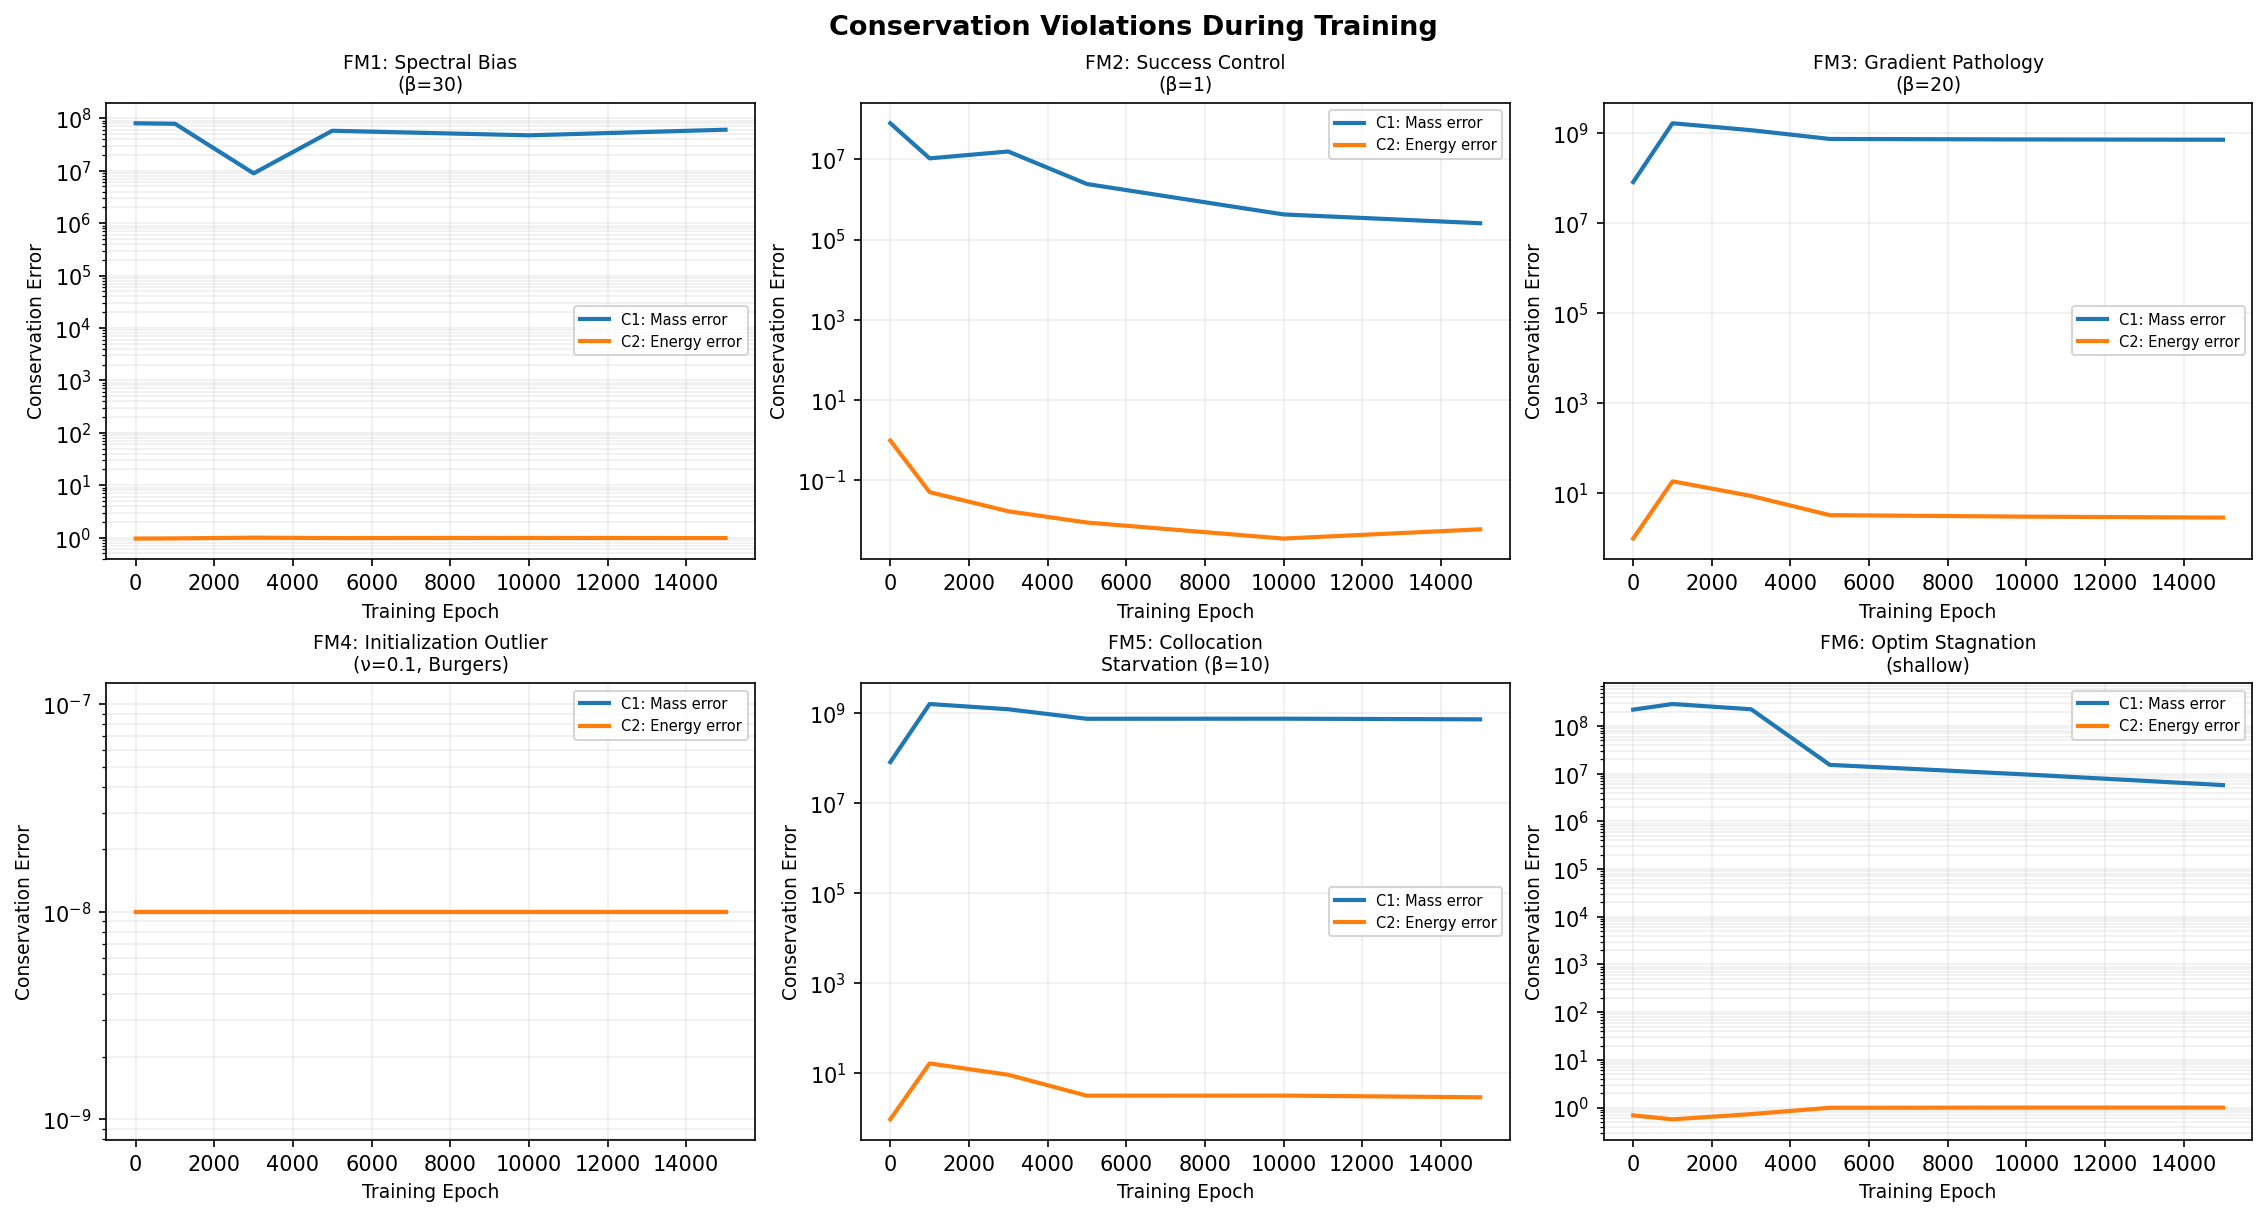
\includegraphics[width=\linewidth]{results/exp26/violation_vs_training.png}
    \caption{Trajectory of macroscopic conservation violations computed over training epochs, showing early physical divergence long before the pointwise $\Ltwo$ error actually stabilizes.}
    \label{fig:exp26_training}
\end{figure}

Tracking these physical invariants dynamically across the training timeline reveals that severe conservation violations systematically appear exceedingly early in training, long before the traditional $\Ltwo$ error visibly plateaus. In the examined failure runs, the $C_1$ and $C_2$ integral violations clearly exceed the acceptable $0.1$ threshold as early as epoch $1500$, while the global aggregate loss metrics falsely imply a healthy, continued learning trajectory. This critical disconnect suggests that evaluating physical invariants could serve as highly sensitive, early-warning diagnostic metrics for impending PINN failure.

\subsection{Conservation Violation Heatmap}

Figure~\ref{fig:exp26_violation_heatmap} presents the conservation violation magnitudes across all six failure mode configurations as a heat map. Each cell reports the mean absolute violation of the corresponding invariant at the final evaluation time $t = T$.

\begin{figure}[htpb]
    \centering
    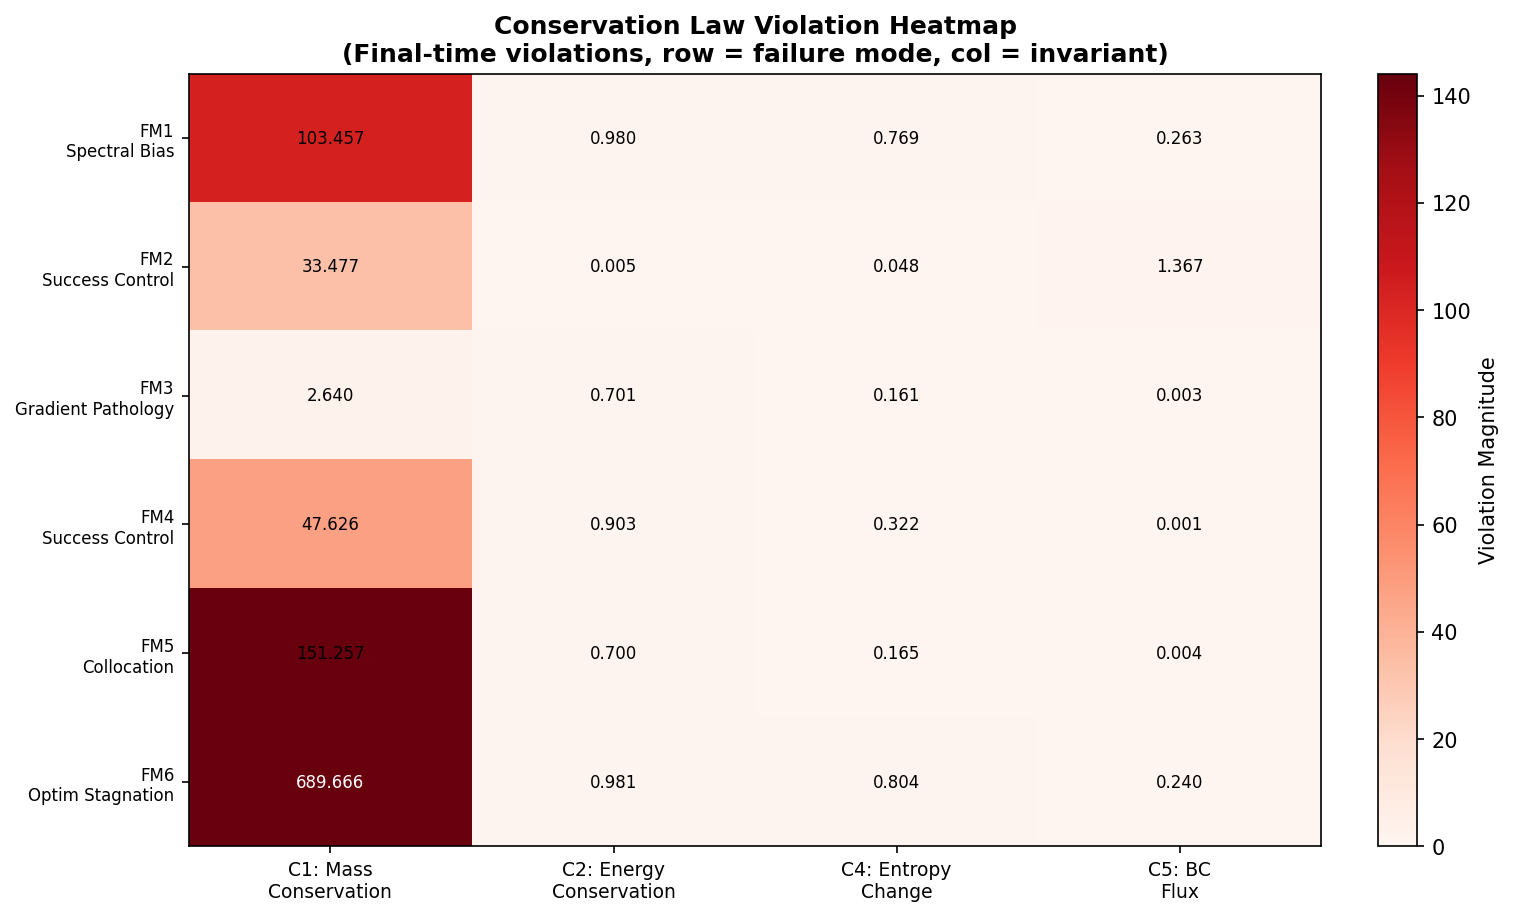
\includegraphics[width=\linewidth]{results/exp26/violation_heatmap.png}
    \caption{Conservation law violation heatmap across all six failure mode configurations (FM1--FM6). Columns report, left to right: $C_1$ (mass conservation violation), $C_2$ (energy conservation violation), $C_3$ (entropy change, a convex entropy functional proxy), and $C_4$ (mean boundary flux leakage). Cell values are final-time violation magnitudes; darker red indicates larger violation. See Table~\ref{tab:exp26_conservation} for the corresponding numerical values for $C_1$ and $C_2$.}
    \label{fig:exp26_violation_heatmap}
\end{figure}
